\section[Quantenmechanik]{Quantenmechanik\footnote{\cite{MRI:quanten}}}
\label{sec:quant}
In diesem Abschnitt wird genauer auf die quantenmechanischen Abl"aufe bei der Magnetresonanztomographie eingegangen, wobei die vorher erl"auterten Grundlagen nur ein klassisches Model sind und wenig mit der Realit"at gemein haben. Die Quantenmechanik erkl"art die realen Abl"aufe.


\subsection{Spin}
Die Grundlagen des Spins sind im Kapitel \ref{chapter:spin} erl"autert. Ein wichtiger Unterschied zur klassischen Physik ist, dass der Spin den Drehimpuls und das magnetische Moment zusammenkoppelt.

Es wird hier gezeigt, wie der Spin eines Wasserstoffatoms in einem Magnetfeld berechnet werden kann. Der daf"ur verwendete Hamilton Operator sieht f"ur ein Elektron wie folgt aus:
\begin{equation}
	H = H_0 + \frac{e}{m_e}\cdot \vec{S} \cdot \vec{B}
\end{equation}
Wobei $\vec{S}$ der Spin ist und $\vec{B}$ das Magnetfeld.

\begin{figure}[h]
	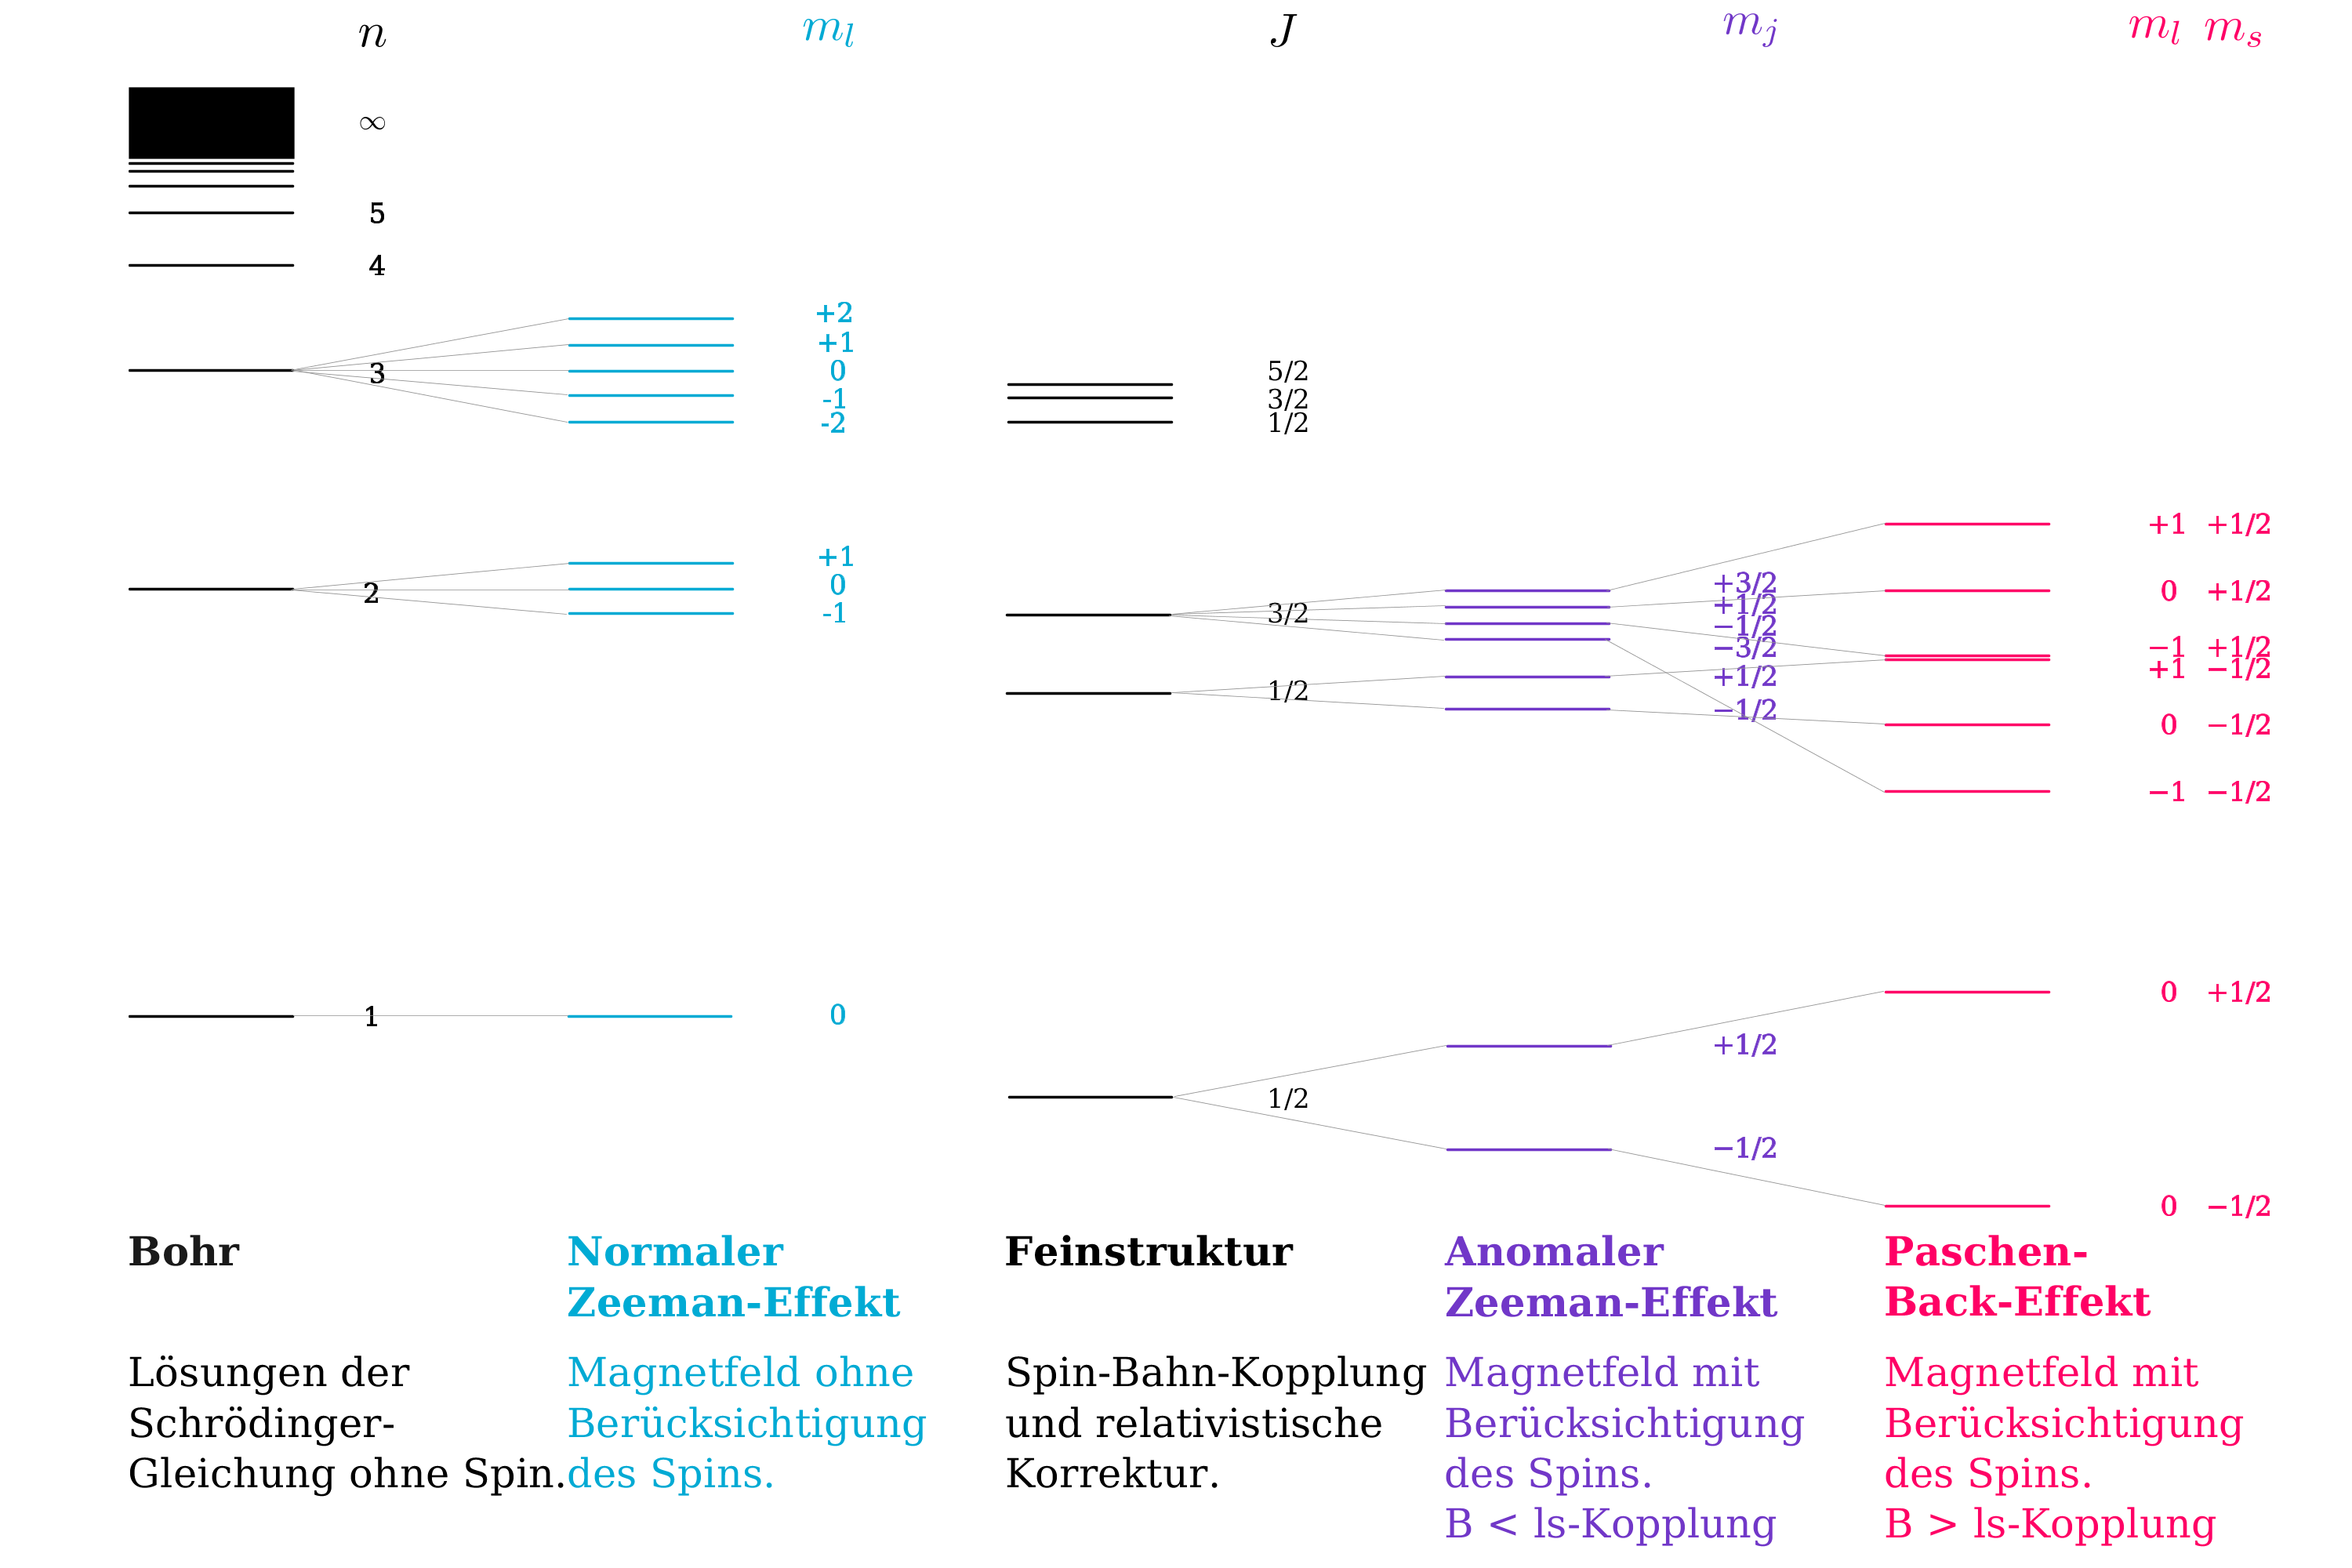
\includegraphics[width = \textwidth]{./mri/pic/index}
	\caption{Aufspaltungen der Wasserstoffniveaus unter Einfluss eines Magnetfeldes \cite{Zeeman}}
	\label{mri:quant:abb:zeeman}
\end{figure}
In dem Kapitel \ref{chapter:atomuhr} wurde auf die Feinstruktur"uberg"ange eingegangen. Die Abbildung \ref{mri:quant:abb:zeeman} zeigt genau diese "Uberg"ange f"ur ein Elektron auf. Da bei der Magnetresonanztomographie aber die Protonen entscheiden sind dient die Abbildung \ref{mri:quant:abb:zeeman} nur als Veranschaulichung des Prozesses. Es wird der Hamiltonoperator f"ur ein Proton ben"otigt, dieser sieht wie folgt aus:
\begin{equation}
H = H_0 + \frac{e}{m_p }\cdot \vec{-S} \cdot \vec{B}
\label{mri:hamilton}
\end{equation}
Der Term $H_0$ beschreibt den Hamiltonoperator ohne der St"orung durch ein Magnetfeld. Er stellt den Grundzustand des Protons dar. Wobei $H_0$ wie folgt definiert ist:
\begin{equation}
H_0 = \frac{\hbar}{2m_p} p^2 + V_p
\end{equation}
Bei $V_p$ handelt es sich um ein Potential, dass die Protonen im Atom an ihrem Platz h"alt.

Bei der Annahme $\vec{B} = \begin{pmatrix}
0 \\
0 \\
B_z \\
\end{pmatrix}$ ergibt sich f"ur den St"orterm $H_1$ folgende Gleichung:
\begin{equation}
H_1 = -\frac{\hbar e}{2m_p} \cdot B_z \begin{pmatrix}
1 & 0 \\
0 & -1 \\
\end{pmatrix}
\end{equation}
Aus diesem St"orterm kann nun mit der Hilfe der St"orungstheorie zwei verschiedenen Energieniveaus berechnet werden.
\begin{equation}
E_\downarrow^{(1)}
=
\langle \downarrow|\, H_1 \,|\downarrow\rangle
=-\frac{\hbar e}{2m_p}
\qquad
E_\uparrow^{(1)}
=
\langle \uparrow|\, H_1 \,|\uparrow\rangle
=\frac{\hbar e}{2m_p}
\end{equation}
Der Energieunterschied ist nun also:
\begin{equation}
\Delta E = \frac{\hbar e}{m_p}B_z
\end{equation}
Der Zusammenhang mit der klassischen Physik ist nun in der Larmorfrequenz  zu finden:
\begin{equation}
\Delta E = \hbar \omega_{\text{Larmor}}=\hbar \gamma B_z
\end{equation}

\subsubsection{Einsteinsche Koeffizienten}
Mit der Hilfe der einsteinschen Koeffizienten kann das Prinzip wie folgt erkl"art werden.
\begin{figure}[h]
	\centering
	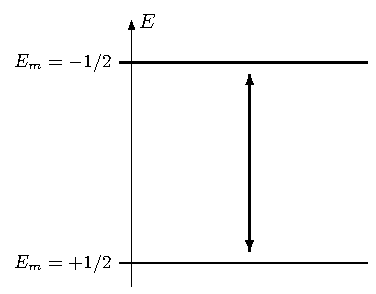
\includegraphics[width= 0.3\textwidth]{./mri/pic/einsteinischeKoeffizienten}
	\caption{"Ubergang $m=+1/2 \longleftrightarrow m=-1/2$}
	\label{mri:relax}
\end{figure}
Betrachtet man die beiden Niveaus $m= -1/2$ und $m= +1/2$ in der Abbildung \ref{mri:relax} f"ur den Kernspin $1/2$ ($^1H$) so findet der einzig m"ogliche Resonanzausgleich zwischen den beiden Energieniveaus statt. 

\subsection{Zeitabh"angige Prozesse}
Zur Erkl"arung der vorg"angig mit der klassischen Physik erl"auterten Relaxationszeiten $T_1$ und $T_2$ werden zeitabh"angige Prozesse ben"otigt. F"ur die Relaxationszeit $T_1$ wird die zeitabh"angige Schr"odingergleichung verwendet:
\begin{equation}
\frac{\hbar}{i} \frac{\partial}{\partial x} |\psi\rangle = H\,|\psi\rangle + \text{Wechselwirkung mit der Umgebung}
\end{equation}
Wobei die zeitabh"angigen Terme folgende sind: "`Wechselwirkung mit der Umgebung"' und "'$H$"'. 
$H$ ist in der Formel \ref{mri:hamilton} ersichtlich, dabei ist der zeitabh"angige Teil im Magnetfeld $\vec{B}$ angesiedelt:
\begin{equation}
\vec{B} = \vec{B_0} + \vec{B}(t)
\end{equation}
Wobei $\vec{B}(t)$ das wechselgerichtete Magnetfeld des Hochfrequenzimpulses ist.

Bei der Wechselwirkung mit der Umgebung handelt es sich um die sogenannte Spin-Gitter-Wechselwirkung. Durch diese Wechselwirkung mit den in der Umgebung des Protons angesiedelten Atomen und Molek"ulen l"asst sich die Relaxationszeit erkl"aren. Die Zeit $T_1$ ist also nicht nur auf das Proton alleine zur"uckzuf"uhren, sondern auch auf die Atome in der Umgebung und dem Hochfrequenzimpuls.

\subsubsection{Relaxationszeit $T_2$}

Die Transversale  Relaxationszeit $T_2$ wird bestimmt durch statistische Gegebenheiten der Protonen. Das heisst, dass die Zeiten mehrerer Protonen ausgewertet werden. Mit der Theorie in diesem Skript kann die Relaxationszeit $T_2$ nicht beschrieben werden. Dazu w"are die Quantenmechanik mehrerer wechselwirkender Teilchen notwendig. 

Zur Veranschaulichung zeigt die Tabelle \ref{mri:quant:tab:zeiten} einige Relaxationszeiten f"ur verschiedene Gewebearten.

\begin{table}[h]
	\centering
		\begin{tabular}{|c|c|c|}
			\hline
			(bei $\vec{B}$ = 1.5 T) & $T_1$ (ms) & $T_2$ (ms) \\
			\hline
			Lunge & 830 & 79 \\
			Leber & 490 & 43 \\
			Milz & 780 & 67 \\
			Niere & 650 & 58 \\
			Fett & 260 & 84 \\	
			\hline	
		\end{tabular}
		\caption{Unterschiedliche Relaxationszeiten verschiedener Gewebearten}
		\label{mri:quant:tab:zeiten}
\end{table}
%TODO Relaxation T_1
%TODO relaxation durch spin-lattice-relaxtion erklären -> Durch die umgebungsatome und deren Feldern wird die Relaxationszeit T_1 beeinflusst sprich definiert.
%
%Zeitabhänigge Schrödinger gleichung aufzeichnen
%Relaxtion T_2 ist zu wenig bekannt es handelt sich um eine statistische berechnung.
%TODO EIne statistische 









%Alle Atome mit einer ungeraden Anzahl von Protonen und/oder Neutronen (z.B. 
%$^1
%H, 
%^13
%C$) besitzen in ihrem Grundzustand einen von Null verschiedenen Kernspin. 
%%Damit ist das Dipolmoment gegeben durch
%%\begin{equation}
%%\vec{\mu}=\gamma \vec{S} = \gamma H \vec{S}
%%\end{equation}
%Ist ein solches kernmagnetisches Moment im Magnetfeld vorhanden, so beobachtet man den Zeeman Effekt. Dieser "aussert sich durch die Aufspaltung der Spektrallinien wie es in der Abbildung \ref{mri:quant:abb:zeeman} ersichtlich ist. In einer ersten N"aherung kann dieser Effekt durch ein ungest"orter, nicht relativistischen Hamilton Operator erkl"art werden. F"ur ein konstantes Magnetfeld in $z$-Richtung sieht dieser wie folgt aus:
%\begin{equation}
%H_{0,z} = -\gamma \vec{B} \vec{S}
%\end{equation}
%
%
%\subsection{Relaxation}
%Unter Relaxation versteht man die Vorg"ange, welche die Kernspin-Magnetisierung in ihren Gleichgewichtszustand zur"uckkehren l"asst, dass ergibt unterschiedliche Relaxationzeiten, welche f"ur die Bildgebung verwendet werden k"onnen. Unterschiedliche Gewebearten ergeben verschiedene Zeiten. Die Tabelle \ref{mri:quant:tab:zeiten} stellt einige Zeiten dar.
%\begin{table}
%	\centering
%		\begin{tabular}{|l|l|l|}
%			\hline
%			(bei B = 1.5 T) & $T_1$ (ms) & $T_2$ (ms) \\
%			\hline
%			Lunge & 830 & 79 \\
%			Leber & 490 & 43 \\
%			Milz & 780 & 67 \\
%			Niere & 650 & 58 \\
%			Fett & 260 & 84 \\	
%			\hline	
%		\end{tabular}
%		\caption{Unterschiedliche Relaxationszeiten verschiedener Gewebearten}
%		\label{mri:quant:tab:zeiten}
%\end{table}
%
%\subsubsection{Prinzip}
%Bei einem Gleichgewicht im Magnetfeld ist die Kernmagnetisierung $\vec{M} = M_0\vec{e_z}$ entlang der Feldrichtung. Die Gr"osse $M_0$ ist durch die Boltzmann-Statistik definiert. Die Magnetiesierungskomponente in $z$-Richtung nennt man longitudinale Magnetisierung. Die Magnetisierungskomponenten in $x$- und $y$-Richtung sind im Gleichgewichtsfall in ihrem Betrag gleich null. Durch eine Einstrahlung eines Hochfrequenzimpulses, wird die $z$-Komponente der Magnetisierung $M_z$ gleich null (bzw. -$M_0$). Zus"atzlich ensteht durch diese St"orung auch ein Kernmagnetisierung in $x$-$y$-Ebene mit dem Betrag $M_\perp \neq M_0$. Die Abbildung \ref{mri:quant:abb:Relaxionszeiten} stellt dies grafisch dar.
%\begin{figure}[h]
%	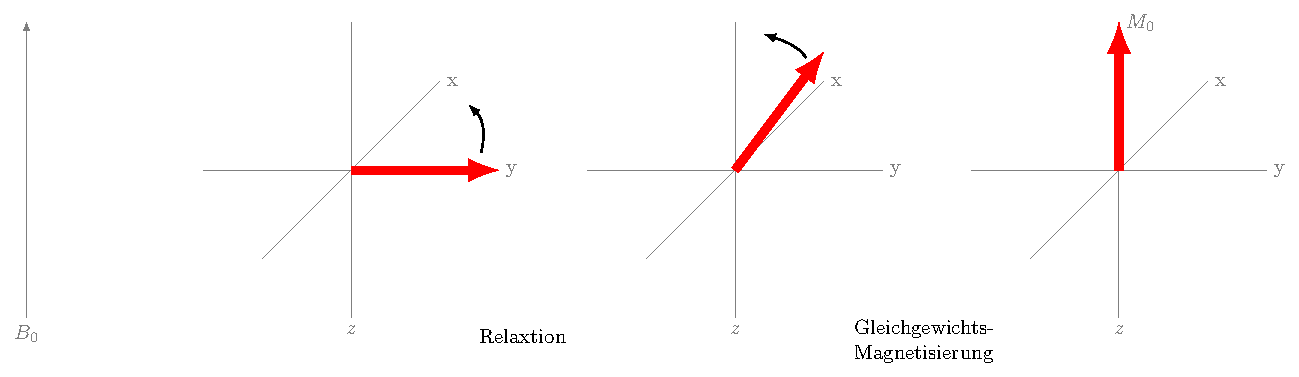
\includegraphics[width= \textwidth]{./mri/pic/relax}
%	\caption{Relaxionszeiten}
%	\label{mri:quant:abb:Relaxionszeiten}
%\end{figure}

%F"ur die Larmorfrequenz der Kernresonanz gilt zumindest oberhalb der Temperatur von einem Kelvin $h v \ll kT$. Deshalb k"onnen die spontanen "Uberg"ange 
%vernachl"assigt werden, und die Wahrscheinlichkeiten f"ur Absorption und induzierte Emission 
%sind gleich.



%\subsubsection{Longitudinale Relaxationszeit $T_1$}
%Die Longitudinale Relaxationszeit ist durch die Zeit $T_1$ definiert. Diese ist definiert durch die Zeit, welche das gest"orte System ben"otigt um in den Gleichgewichtszustand zur"uckzukehren. Dies wird dadurch erreicht, dass das System an die Umgebung Energie verliert.
%\begin{figure}[H]
%\caption{Longitudinale Relaxationszeit $T_1$}
%\label{mri:quant:abb:long}
%\end{figure}

%\subsubsection{Transversale  Relaxationszeit $T_2$}
%Die transversale Relaxationszeit ist durch die Zeit $T_2$ definiert. Sie beschreibt das zeitliche Verhalten der Magnetisierung in der $x$-$y$-Ebene. 
%\begin{figure}[H]
%	\caption{Transversale Relaxationszeit $T_1$}
%	\label{mri:quant:abb:trans}
%\end{figure}

